\section*{Results}
\subsection*{GWAS on the latent representation}
\label{subsec_GWAS}


The comparison of the outcome of GWAS performed on PCA- and CoMA-derived features reveals that the latter method encounters several significant associations with the genotype; in contrast, PCA, despite its comparable reconstruction performance, yields none. % In other words, CoMA allows extracting phenotypes with some level of heritability. 
CoMA experiments and subsequent GWAS were carried out using scaled and unscaled meshes. In both cases, results for $n_z=8$ are reported in the main text. Our results suggest that the Kullback-Leibler regularisation term in the loss function is effective when it comes to obtaining an interpretable low-dimensional representation, by keeping the correlation between different latent variables low. 

\begin{figure*}[ht!]
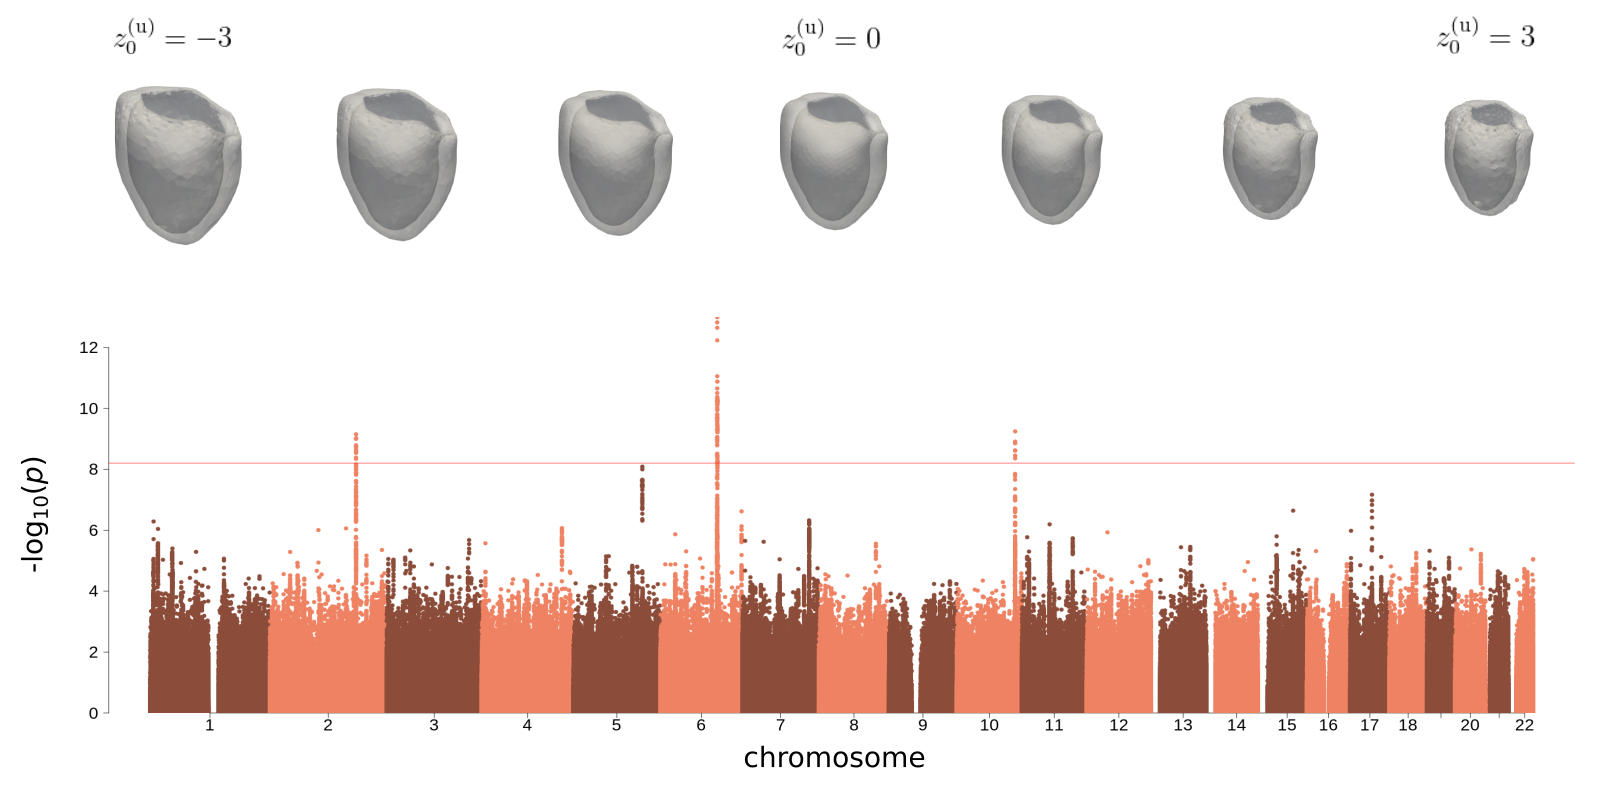
\includegraphics[width=\textwidth]{figs/gwas/GWAS_Experiment2_z0u_unscaled_meshes.png}
\label{fig:manhattan_LV_latent_unscaled}
\caption{Manhattan plot for LV latent variable $z_0^{(\text{u})}$ along with a set of synthetic LV shapes produced by making $z_i=\lambda \delta_{i1}$ for $\lambda\in\{0, \pm 1, \pm 2, \pm 3\}$. Changes in this variable were found to associate with different mitral orientations.}
\end{figure*}


% UNSCALED MESHES
For unscaled meshes (i.e. meshes preserving the original scale from the images), several genome-wide significant associations were found, after further adjusting the $p$-value threshold for the number of latent variables tested ($n_z=8$ in this case). All these associations belonged to a single latent variable, which we will call $z_0^{(\text{u})}$. The Manhattan plots and synthetic shapes produced by varying $z_0^{(\text{u})}$ around the mean shape are displayed in figure \ref{fig:manhattan_LV_latent_unscaled}. Visual inspection of the effect of varying $z_0^{(\text{u})}$ on the reconstructed LV shape indicates that this latent variable controls the size of the LV. 

In order to further characterise this and the rest of the latent variables found, their Spearman correlation with several cardiac indices was computed. These quantities were derived from the cardiac 3D meshes. Details are explained in the supplementary material. It can be seen that Spearman correlation of LVEDV and $z_0^{(\text{u})}$ is almost perfect (\textcolor{red}{how much}).

The locus at chromosome 2 ($p=10^{-10}$) has been reported in  \cite{ref_nayaung, ref_pirruccello} and mapped to gene TTN. This gene encodes for protein titin, which is  responsible  for  the  sarcomere  assembly of the myocytes, which in turn determines stretching, contraction and passive stiffness of the myocardium \cite{granzier_giant_2004}.

Therefore, this method, applied to unscaled meshes, allows to retrieve prior knowledge on the genetic basis of LV size.

For scaled meshes, 

Spearman correlation of latent variables with demographic data was computed and is displayed in figure \ref{fig:relation_to_demographic}.
Interestingly, for scaled meshes, latent variable $z_1^{(s)}$ is significantly correlated with DBP, SBP, BMI and sex (but not with height), whereas latent variable $z_5$ (linked with PLN) is not strongly linked with any demographic variable.
A $t$-test was conducted to determine whether the latent variables were significantly different for subjects with specific cardiac diseases, as compared to people without such diagnoses. To do this, ICD10 codes provided by the UK Biobank were used. The results are presented in \ref{fig:health_outcomes}.

% SCALED MESHES

variational CoMA yielded a latent variable, which we will call $z_0^{(\text{s})}$, with a single Bonferroni-significant genetic locus in chromosome 6 ($p=10^{-17}$). The associated Manhattan plots are shown in figure \ref{fig:manhattan_LV_latent}, along with the corresponding change in shape produced by the latent variable tested. The morphological impact of $z_0^{(\text{s})}$ is associated with LV sphericity index (see following subsection), as can be seen both by visual inspection of \ref{fig:manhattan_LV_latent} and from the Spearman correlation coefficient in figure \ref{fig:relation_to_indices}.

%(sarco/endoplasmic reticulum Ca$^{2+}$-ATPase)which transports calcium from the cytosol into the SR1. 
%In its dephosphorylated state, PLN lowers the affinity of SERCA for Ca$^{2+}$, thereby inhibiting calcium uptake. Phosphorylation of PLN at serine 16 by PKA (protein kinase A) or threonine 17 by CaMKII (Ca$^{2+}$/calmodulin-dependent protein kinase II) relieves PLN-mediated inhibition of SERCA, thereby increasing SERCA activity and subsequent uptake of calcium. 
Again, we have been able to map this genetic association to gene PLN (phospholamban) with high confidence, based on the literature on genetics of cardiac phenotypes. 
PLN plays a crucial role in cardiomyocyte calcium handling by acting as a primary regulator of the SERCA protein (sarco/endoplasmic reticulum Ca$^{2+}$-ATPase), which transports calcium from the cytosol into the SR1. In its dephosphorylated state, PLN lowers the affinity of SERCA for Ca$^{2+}$, thereby inhibiting calcium uptake. Phosphorylation of PLN at serine 16 by PKA (protein kinase A) or threonine 17 by CaMKII (Ca$^{2+}$/calmodulin-dependent protein kinase II) relieves PLN-mediated inhibition of SERCA, thereby increasing SERCA activity and subsequent uptake of calcium. The PLN-SERCA interaction is essential for contraction and relaxation of the heart, and is under the regulation of the $\beta$-adrenergic receptor pathway to adapt cardiac output to physiological needs. \cite{maclennan_2003}

\begin{figure*}[ht!]
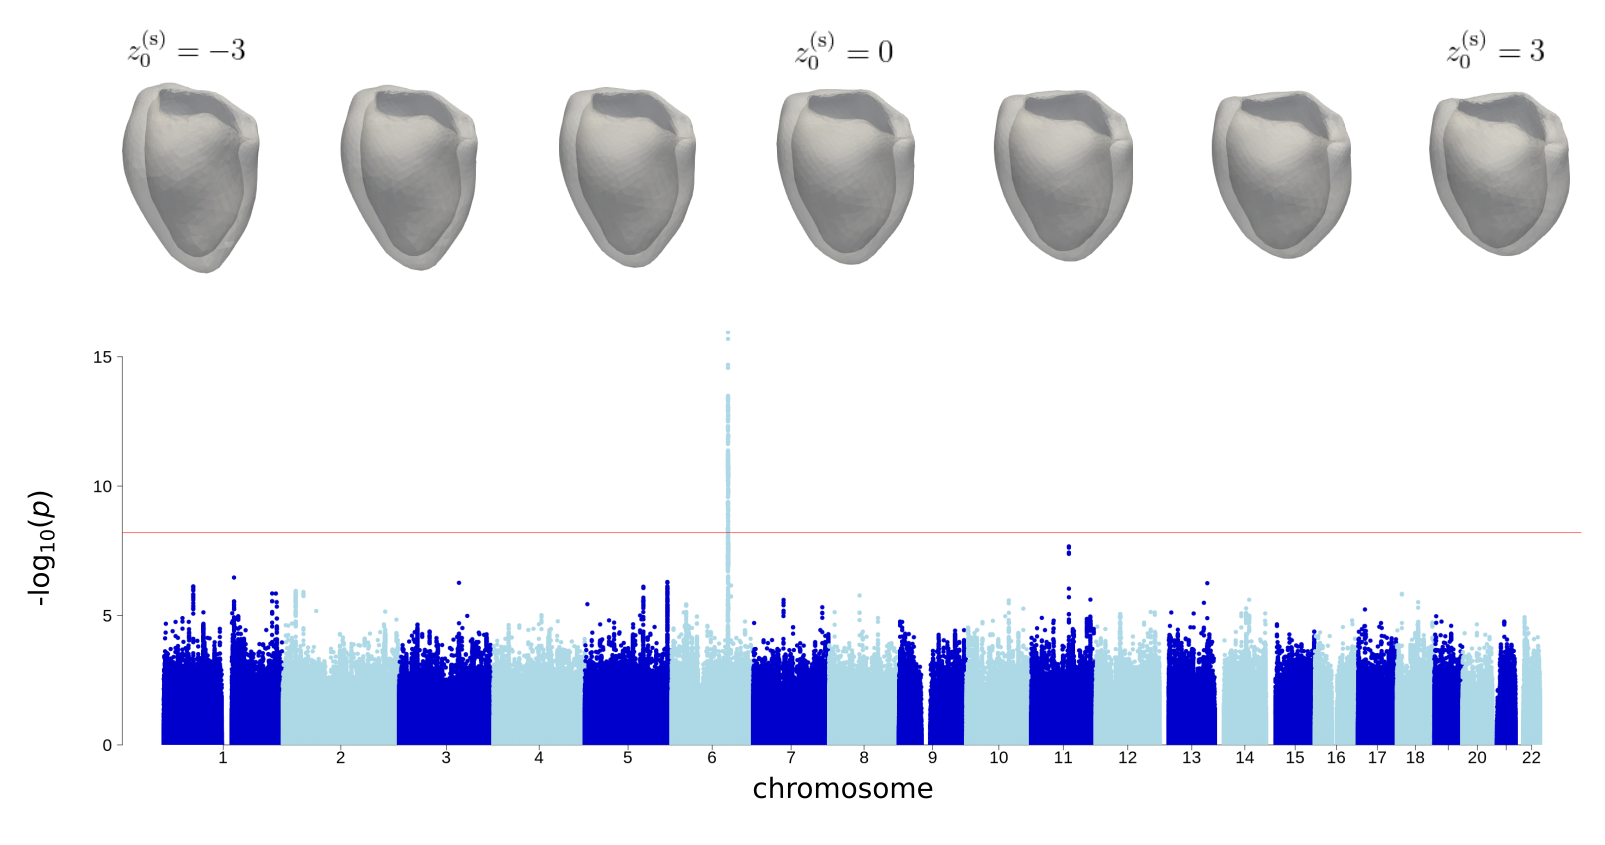
\includegraphics[width=\textwidth]{figs/gwas/GWAS_Experiment1_z0s_scaled_meshes.png}
\caption{Manhattan plot for LV latent variable $z_0^{(\text{s})}$ along with a set of synthetic LV shapes produced by making $z_i=\lambda \delta_{i0}$ for $\lambda\in\{0, \pm 1, \pm 2, \pm 3\}$. This latent variable showed to be associated to LV sphericity index.}
\label{fig:manhattan_LV_latent}
\end{figure*}

Mutations in PLN have a well-established relationship with dilated cardiomyopathy (DCM) \cite{ref_Eijgenraam}. Besides two recent studies, also on UKB data, \cite{ref_pirruccello}, to the best of our knowledge this gene had not been reported in a GWAS of non-disease phenotypes. In \cite{ref_pirruccello}, PLN was found to be associated with LV end-diastolic and end-systolic volumes (LVEDV and LVESV). Interestingly, latent variable $z_0^{(\text{s})}$ yielded a $p$-value lower than the associations reported therein ($10^{-16}$ and $10^{-10}$ for LVEDV and LVESV, respectively). Also, the PLN locus was the only association found for $z_0^{(\text{s})}$, whereas for LV volumes the number of independent genome-wide significant associations is much higher. 

The hypothesis that the PLN association with LV volume is actually mediated by a morphological change captured by $z_0^{(\text{s})}$ was tested. To do this, LV volume was tested in GWAS after being adjusted for $z_0^{(\text{s})}$ as a covariate, however the PLN association remained significant (see supplementary material), suggesting that PLN controls these two phenotypes independently. Consistent with this conclusion, it can be seen that $z_0^{(\text{s})}$ does not correlate with LV size (see )

Also interestingly, the shape variation associated with high positive values of $z_0^{(\text{s})}$ follows the usual cardiac remodelling linked to DCM \cite{ref_dcm}. Despite the low number of DCM cases within our UKB subcohort (21 subjects), conducting a $t$-test on $z_0^{(\text{s})}$ between individuals with a DCM diagnosis and without, showed that the mean of $z_0^{(\text{s})}$ is significantly different between the two groups ($p=10^{-3}$) (see)

\begin{figure}[ht!]
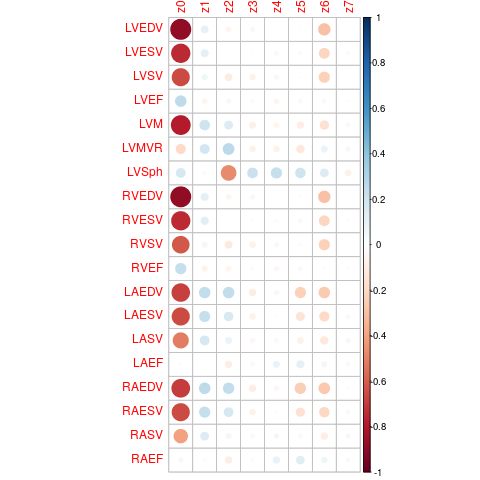
\includegraphics[width=0.5\textwidth]{figs/correlation/experiment_2_vs_cardiac_indices}
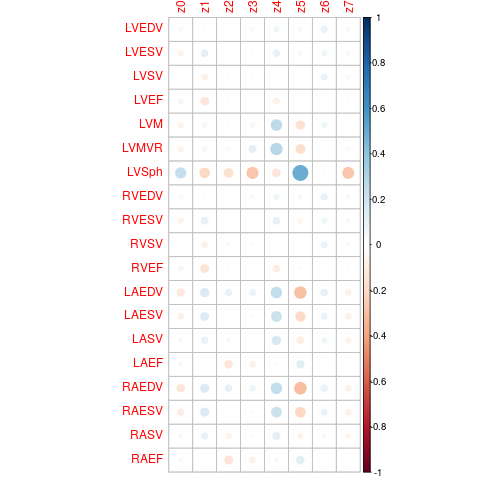
\includegraphics[width=0.5\textwidth]{figs/correlation/experiment_1_vs_cardiac_indices}
\caption{Spearman correlation of the latent variables with traditional cardiac indices for all the cardiac chambers, for CoMA experiments performed on a) unscaled and b) scaled cardiac meshes. XEDV and XESV stand for end-diastolic and end-systolic volume, respectively, whereas $\text{XSV}=\text{XEDV}-\text{XSV}$ and $\text{XEF}=\text{XSV}/\text{XEDV}$ are the stroke volume and the ejection fraction, respectively, where X is one of LV, RV, LA or RA. Finally, LVM stands for LV myocardial mass, whereas $\text{LVMVR}=\text{LVM}/\text{LVEDV}$ is the myorcardial-mass-to-volume ratio and LVSph is LV sphericity index.)}
\label{fig:relation_to_indices}
\end{figure}


\begin{figure}[ht!]
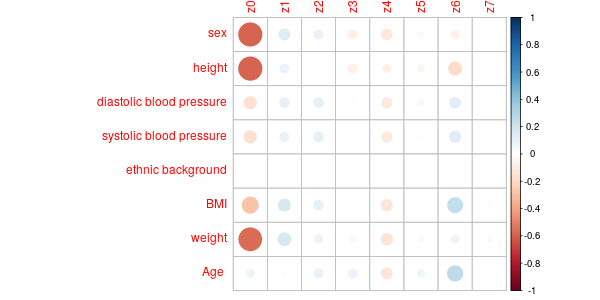
\includegraphics[width=0.5\textwidth]{figs/correlation/experiment_2_vs_demographic_data}A
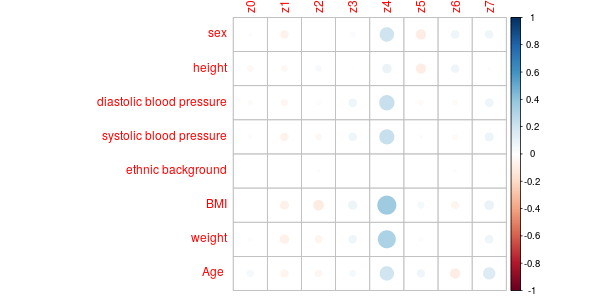
\includegraphics[width=0.5\textwidth]{figs/correlation/experiment_1_vs_demographic_data}B

\caption{Spearman correlation of the latent variables with demographic data for all the cardiac chambers, for CoMA experiments performed on a) unscaled and b) scaled cardiac meshes.}
\label{fig:relation_to_demographic}
\end{figure}



%\subsection*{Heritability analysis}
%\textcolor{gray}{Run LD-score regression or GCTA-GREML to estimate heritability of the latent features.}

% \subsection*{Transcriptome-wide associations studies (TWAS)}
